\chapter{Data Preprocessing}
  \section{Introduction}
    It is typical to apply some sort of preprocessing operations to any data fed into
    a neural network. Although in theory a neural network can learn very complex
    non-linear transformations, it is often the case that learning this at the same
    time as learning other abilities is unrealistic. Preprocessing methods can
    also embed information about the dataset into each frame which the network is
    unlikely to learn as it works on a per example basis (this is a motivation for
    recurrent networks).
     Therefore it is vital to try
    different pre-processing methods on the data.
    Recalling of the aims of this project it is also vital to try a range of methods
    because only a few
    might allow the autoencoder and classifier structures to cooperate with each other.
    This section describes some preprocessing methods which are to be
    tested in section \ref{sec:psearch}.

    % You should mention how: by a piece-wise
    % affine warp of the triangulated landmarks to a canonical shape.
    % And why: so that the facial regions within different
    % frames are aligned with each other, so that the network
    % does not need to account for spatial variations.

    The DISFA dataset as described in section \ref{disfa_list} has frames of size $ 1024 \times 764 $
    but using previous work of Sebastian Kaltwang\cite{Kaltwang2015} faces are
    centred and normalised by a piece-wise affine warp of the triangulated
    landmarks to a canonical shape to give an image of size $118 \times 128$
    with pixels being integers between
    0 and 255. An illustration is shown in figure \ref{fig:sebproc}.
    This is done in order to align face images with each other so that
    there is no need for the model to account for spatial variations.

    \begin{figure}[!h] \centering
    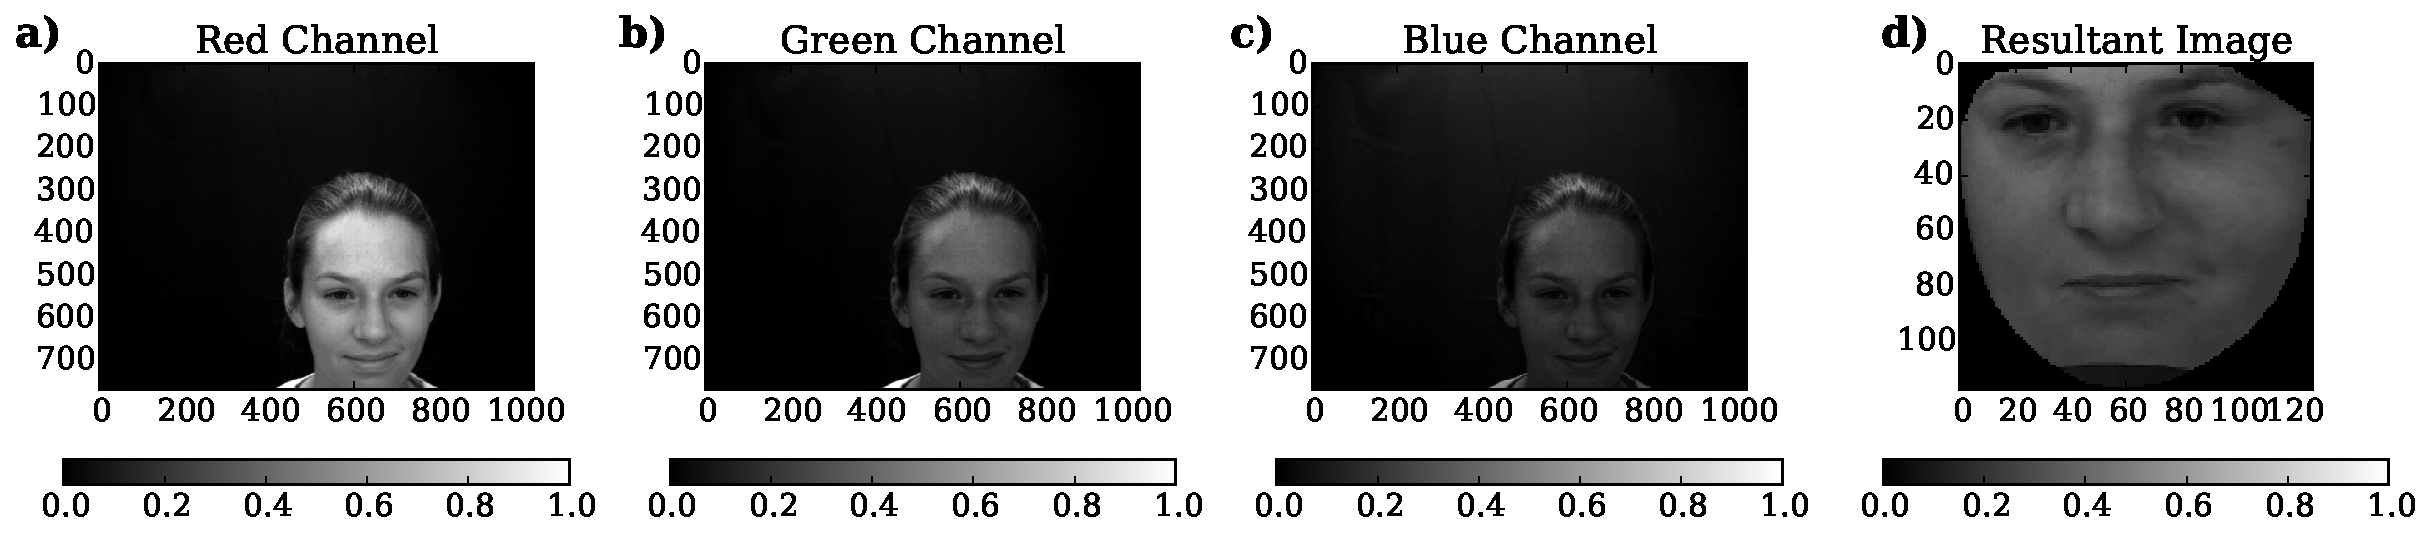
\includegraphics[width =\hsize]{figures/seb_preproc.pdf}
    \caption{ {\bf a) b) c)} An example of the original $764 \times 1024$ image with
    the 3 RGB channels displayed separately. {\bf d)} the resultant image
    $118 \times 128$ after face registration.} \label{fig:sebproc} \end{figure}


    This section first discusses the initial treatment of the labels.
    Then three different methods of normalising and scaling
    the dataset are described, these can be combined to create further methods. In order to illustrate
    the effect of such operations figures such as figure \ref{fig:faces_none} are used which
    show an example face and some statistically generated faces. The ideal method will
    have minimum and maximum faces which express high degrees of facial expression, so that
    high pixel values can easily be correlated to various AUs in the classifier. Another motivation
    for trying this many methods is to improve the chances of finding an input format which works will with both an
    autoencoder and classifier.

    \section{Methods For Labels}

      Labels are defined as a matrix:
      \begin{equation}
        {\bf y} \in \{0,1,2,3,4,5\}^{N\times F}
      \end{equation}

      Where $F$ is the number of AUs and $N$ is the number of labelled images
      in the dataset.

      Five is the highest intensity for an AU and zero is the absence of that AU.
      Typically a neural network outputs values between zero and one so these values are divided by five to make them compatible.
      For an intensity estimation problem that is all that is required, however for classification
      the AU labels need to be binary so a threshold is chosen at which an AU is considered present.
      Finally in the case of the Binary Softmax described in section \ref{sec:binsoft} the label vector
      needs to be expanded to also contain the negative case, hence doubling its size.

  \section{Methods For Images} \label{sec:methods}

    \begin{figure}[!h] \centering
    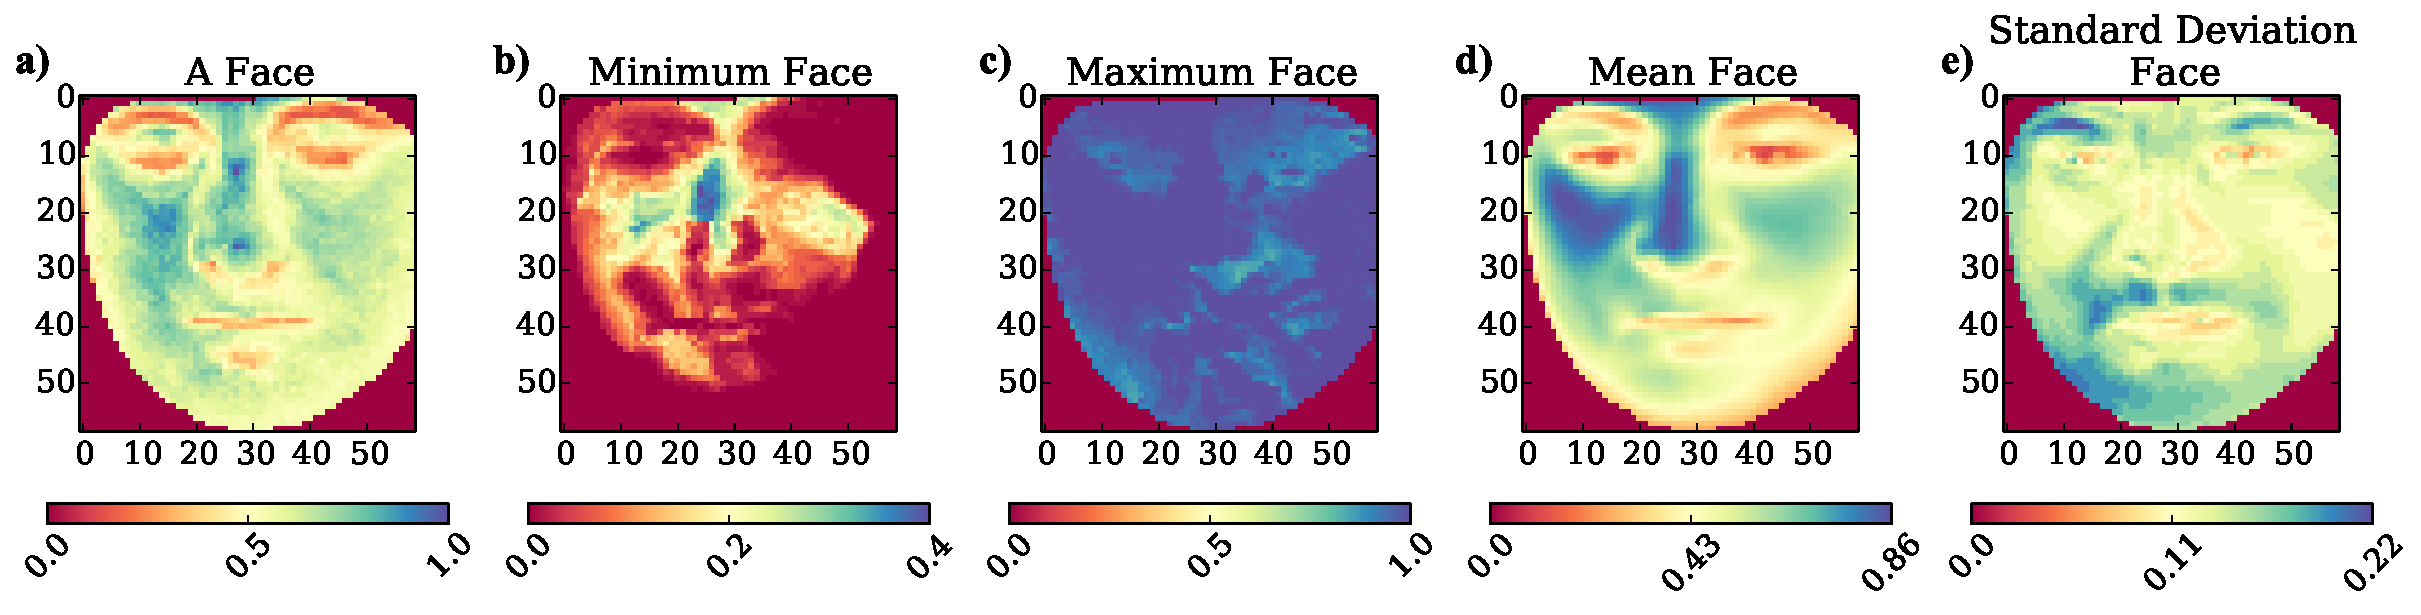
\includegraphics[width =\hsize]{figures/faces.pdf}
    \caption{The DISFA dataset with no preprocessing, it shows
    the images at the last stage of figure \ref{fig:sebproc}.
    Plots {\bf a)}, {\bf b)}, {\bf c)}, {\bf d)} and {\bf e)}
    correspond to a sample face, the minimum, the maximum,
    the mean and the standard deviation values of each pixel across
    the whole dataset respectively. The images were downscaled by a factor of 0.8 before being processed.}
    \label{fig:faces_none} \end{figure}

    The preprocessing methods assume that a dataset of a number of subjects
    is described as a matrix of the form:
    \begin{equation}
    {\bf x} \in \mathbb{R}^{N\times X \times Y},\quad {\bf y} \in \mathbb{N}^{N\times F}
    \end{equation}
    Where $\mathbf{x}$ contains the images, $\mathbf{y}$ contains the labels,
    $N$ is the number of images, $X$ is the width of the image, $Y$ is the height of the
    image and $F$ is the number of AUs labelled. Furthermore in some cases an extra dimension
    for the subject may be added:
    \begin{equation}
    {\bf x} \in \mathbb{R}^{S\times N\times X \times Y},\quad {\bf y} \in \mathbb{N}^{S\times N\times F}
    \end{equation}
    Some subjects may have a slightly different number of frames and this is reflected
    in the implementation but not in this section.

    Each preprocessing method will be denoted by a function ${\bf P}$ defined as follows:
    \begin{equation}
      {\bf P}({\bf x},i) = {\bf x'}_i
    \end{equation}
    For the per subject case:
    \begin{equation}
      {\bf P}({\bf x},i,s) = {\bf x'}_{si}
    \end{equation}
    Where $i$ indexes frames so has $0 \leq i < N$, where $N$ might be the number of frames
    in the whole dataset or just for a subject.

    This notation aims to express the fact that each image in the resultant dataset
    may use information from all other frames, as it is generated by a function of the dataset
    and it's own index $i$.

    %
    %
    %
    %
    %
    \subsection{Contrast Normalisation}
      \begin{figure}[!h]
      \centering
      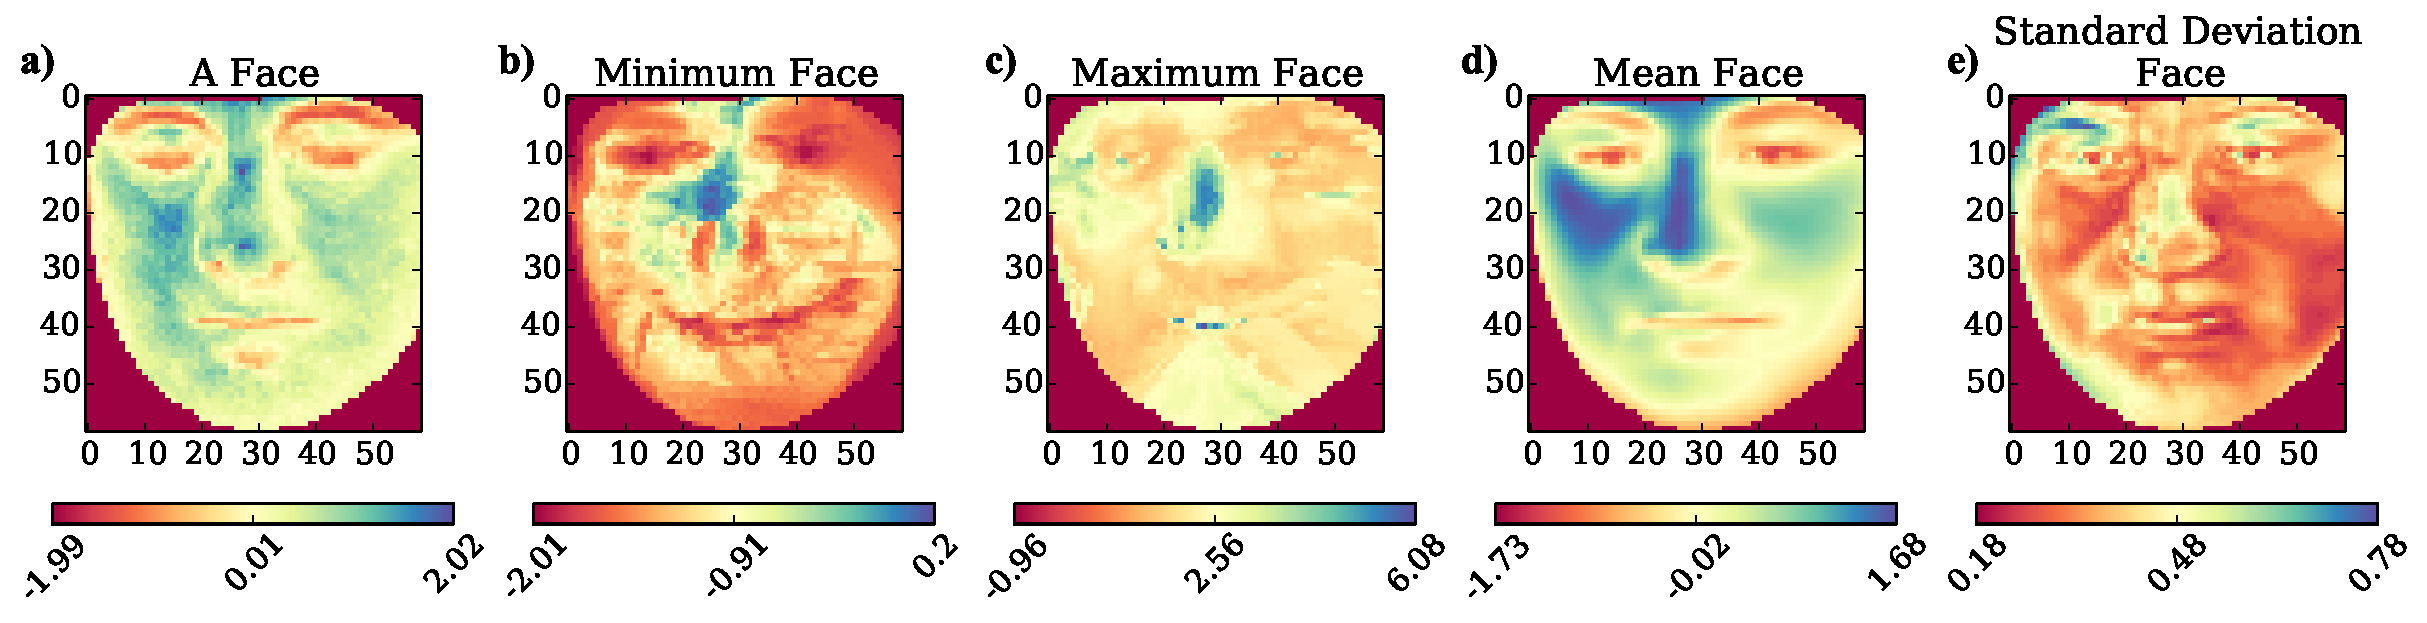
\includegraphics[width =\hsize]{figures/faces_contrast.pdf}
      \caption{The DISFA dataset with {\bf contrast normalisation}.
      Plots {\bf a)}, {\bf b)}, {\bf c)}, {\bf d)} and {\bf e)}
      correspond to a sample face, the minimum, the maximum,
      the mean and the standard deviation values of each pixel across
      the whole dataset. The images were downscaled by a factor of 0.8 before being processed.}
      \label{fig:simple}
      \end{figure}

      For each image find the mean pixel value and standard deviation and then subtract the mean
      and divide by the standard deviation. This standardises the amount of contrast in each image.
      \begin{equation}
         P({\bf x},i)= ({\bf x}_{i} - \mu({\bf x}_{i}))/\sigma ({\bf x}_{i}) = {\bf x}_{i}'
         \label{eq:con}
      \end{equation}
      Where $\mu$ and $\sigma$ gives the mean and standard deviation value of a matrix respectively.
      Equation \ref{eq:con} shows this, a disadvantage of this normalisation is that it
      has no regard of facial structures.

    %
    %
    %
    %
    %
    \subsection{Mean Face Normalisation} \label{sec:meanface}
      Here the mean face and standard deviation face is subtracted and divided away from the
      image, these faces might be per subject or per dataset, as shown:
      \begin{equation}
        P({\bf x},i) =  ({\bf x}_{i} - {\boldsymbol \mu}_0( {\bf x}))/{\boldsymbol \sigma}_0({\bf x}_{i})  = {\bf x}_{i}'
      \end{equation}
      \begin{equation}
        P_s({\bf x},s,i) = ({\bf x}_{si} - {\boldsymbol \mu}_{0}( {\bf x}_s))/{\boldsymbol \sigma}_{0}( {\bf x}_s))  = {\bf x}_{si}'
      \end{equation}
      Where ${\boldsymbol \mu}_{i,j..}$ denotes the mean over the axes $i,j..$ and
      similarly for ${\boldsymbol \sigma} $ the standard deviation.
      The point of this normalisation is to enhance the intensity of any pixels which
      are unusual, these pixels should hold most information about potential facial expressions.
      \begin{figure}[!h] \centering
      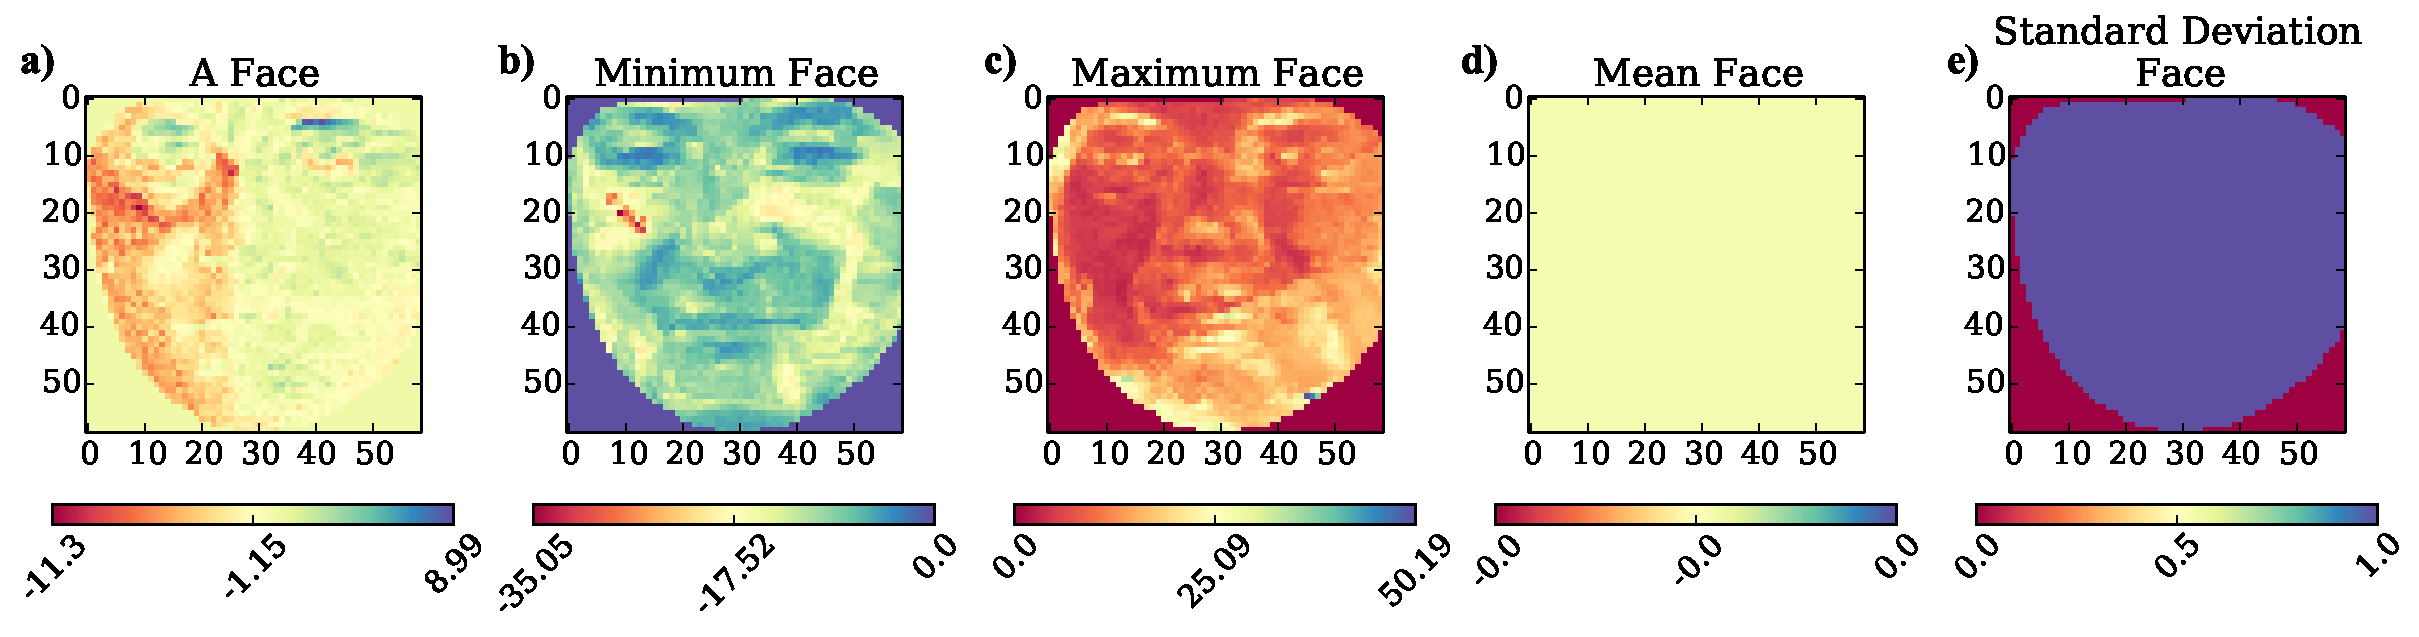
\includegraphics[width =\hsize]{figures/faces_per_subject_face.pdf}
      \caption{The DISFA dataset with {\bf per subject mean face normalisation}.
      Plots {\bf a)}, {\bf b)}, {\bf c)}, {\bf d)} and {\bf e)}
      correspond to a sample face, the minimum, the maximum,
      the mean and the standard deviation values of each pixel across
      the whole dataset. The images were downscaled by a factor of 0.8 before being processed.}
      \label{fig:}
      \end{figure}

    %
    %
    %
    %
    %
    \subsection{Range Scaling}
      This normalisation gets the data between the range of -1 and 1.
      \begin{equation}
        {\boldsymbol r}({\bf x})_{axis} = {\boldsymbol \min}_{axis}({\bf x}) - {\boldsymbol \min}_{axis}({\bf x})
      \end{equation}
      \begin{equation}
         P({\bf x},i) =
         \frac{{\bf x}_{i} - \frac{1}{2}\left ( {\boldsymbol \min}_0({\bf x}) + {\boldsymbol \min}_0({\bf x}) \right ) }{\frac{1}{2}{\boldsymbol r}_0({\bf x})}
         = {\bf x}_{i}'
      \end{equation}
      For the per subject case:
      \begin{equation}
         P_s({\bf x},i,s) =
         \frac{{\bf x}_{si} - {\boldsymbol \min}_0({\bf x}_s) - \frac{1}{2}{\boldsymbol r}_0({\bf x}_s) }{\frac{1}{2}{\boldsymbol r}_0({\bf x}_s)}
         = {\bf x}_{si}'
      \end{equation}
      \begin{figure}[!h] \centering
      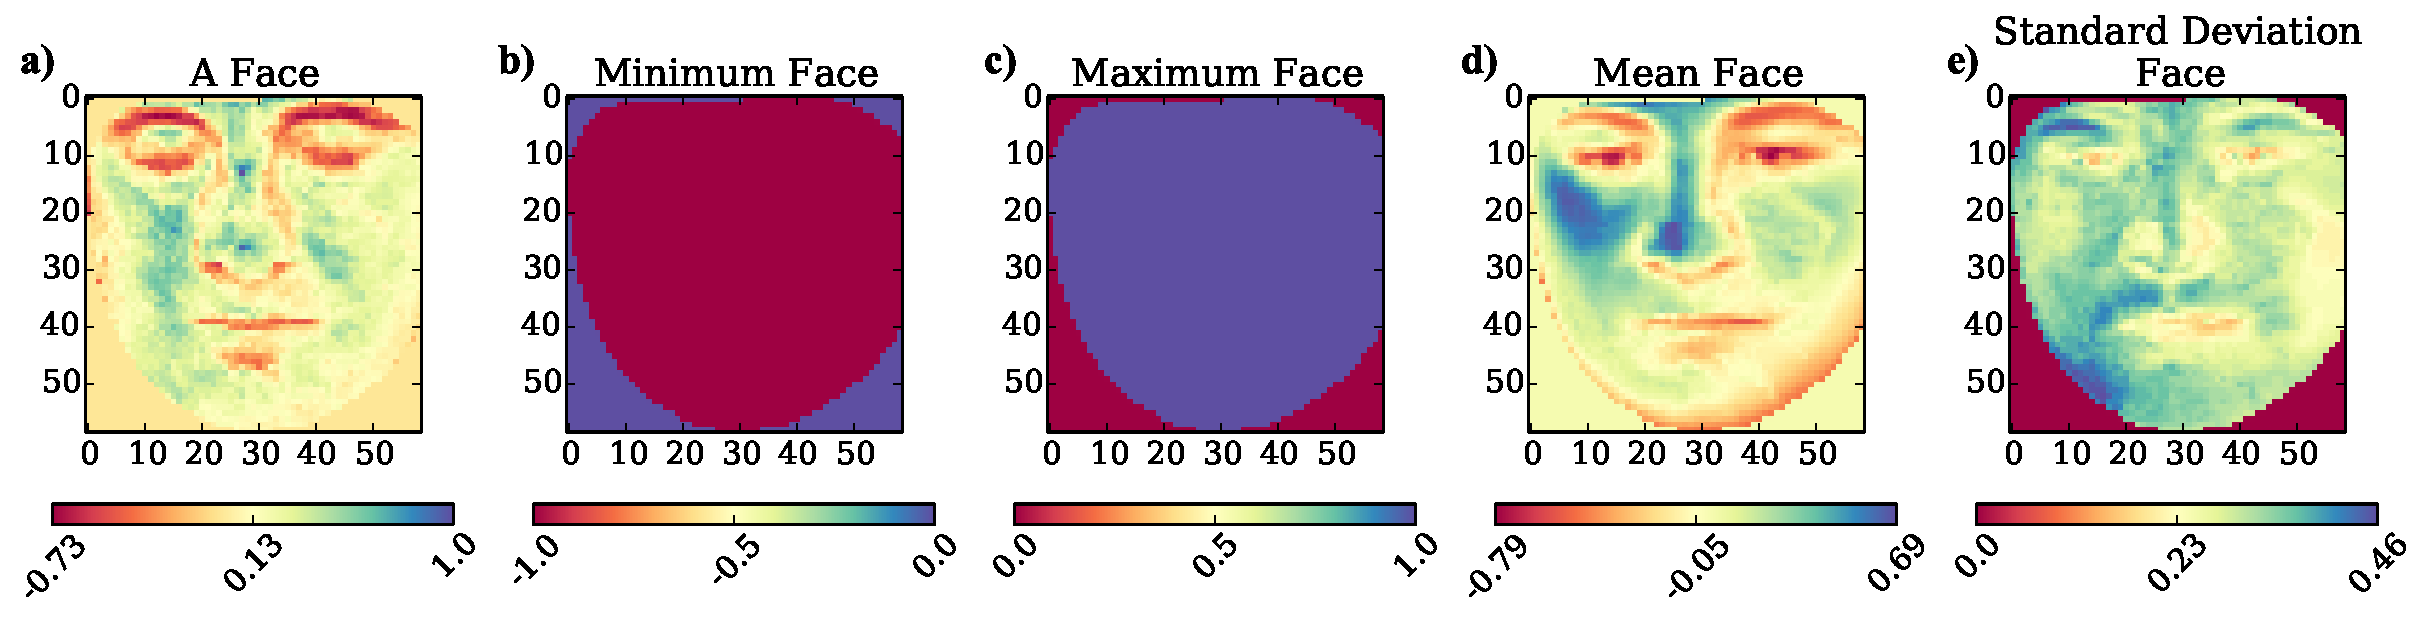
\includegraphics[width =\hsize]{figures/faces_range.pdf}
      \caption{The DISFA dataset with {\bf range scaling between -1 and 1}.
      Plots {\bf a)}, {\bf b)}, {\bf c)}, {\bf d)} and {\bf e)}
      correspond to a sample face, the minimum, the maximum,
      the mean and the standard deviation values of each pixel across
      the whole dataset. The images were downscaled by a factor of 0.8 before being processed.}
      \label{fig:simple} \end{figure}

    %
    %
    %
    %
    %
    \subsection{Combining methods}
      Some methods can be combined, figures \ref{fig:faces_contrast_face} and \ref{fig:faces_per_subject_contrast_face}
      shows the result of combining the mean face subtraction and then the
      contrast normalisation (in the per subject and whole set cases respectively). It is clear the effect is to
      reduce the range of the data, which may be useful for the classifier, however parts of the image
      which were all zero are now not which may result in lower performance.

      \begin{figure}[!h] \centering
      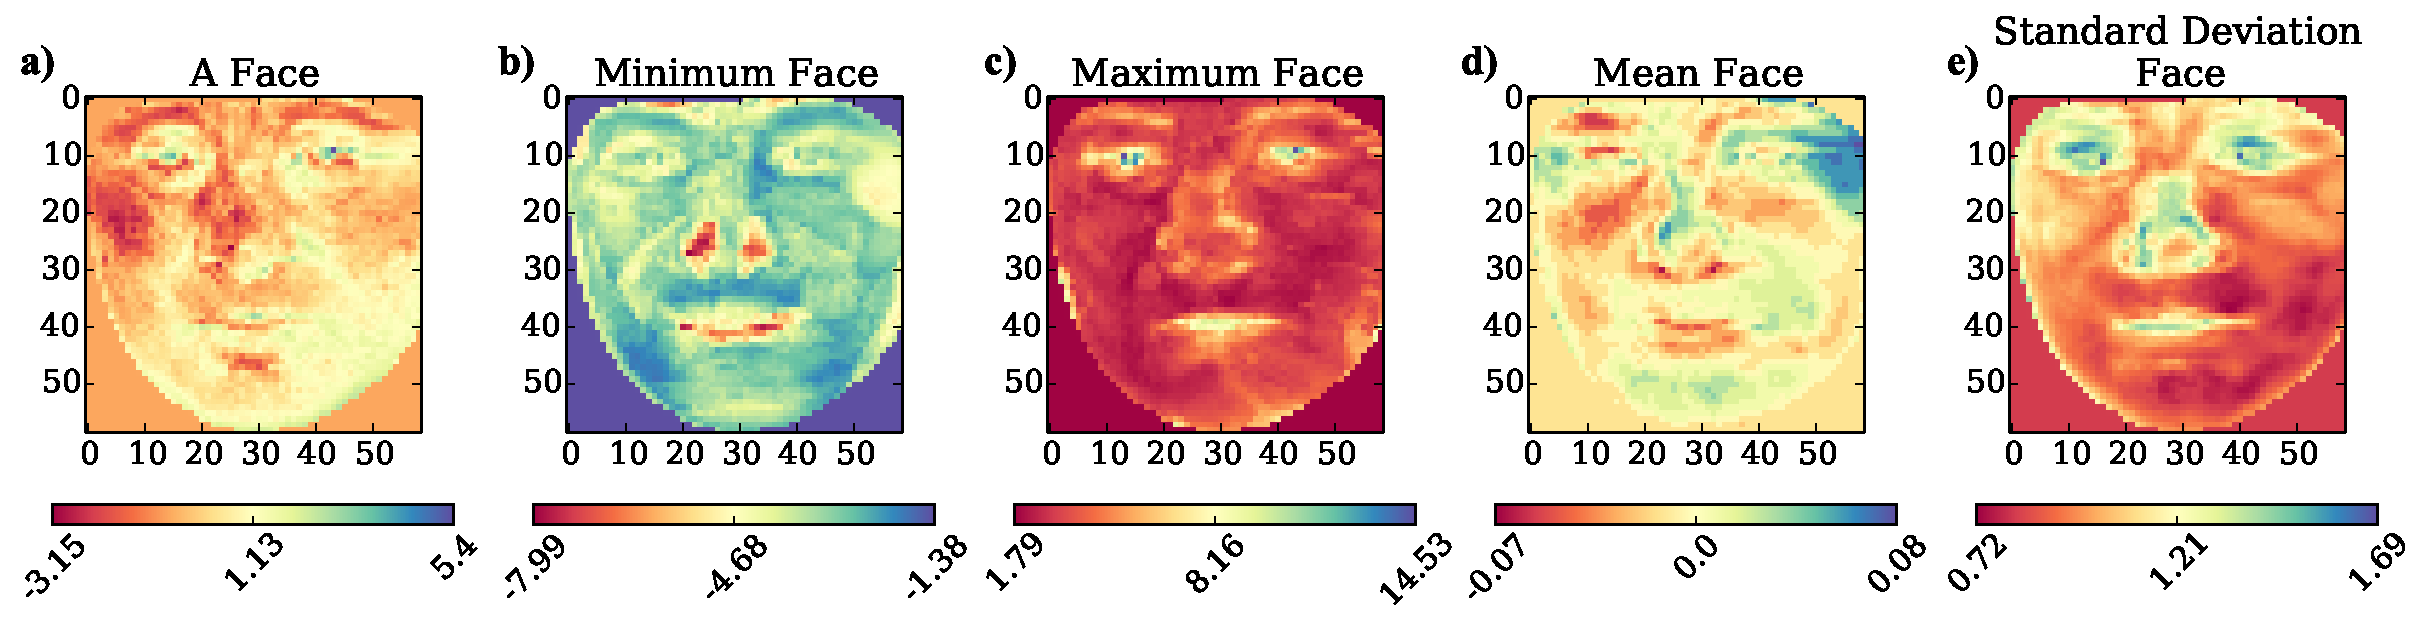
\includegraphics[width =\hsize]{figures/faces_contrast_face.pdf}
      \caption{The DISFA dataset with {\bf mean face normalisation and then contrast normalisation} applied.
      Plots {\bf a)}, {\bf b)}, {\bf c)}, {\bf d)} and {\bf e)}
      correspond to a sample face, the minimum, the maximum,
      the mean and the standard deviation values of each pixel across
      the whole dataset. The images were downscaled by a factor of 0.8 before being processed.}
      \label{fig:faces_contrast_face} \end{figure}

      \begin{figure}[!h] \centering
      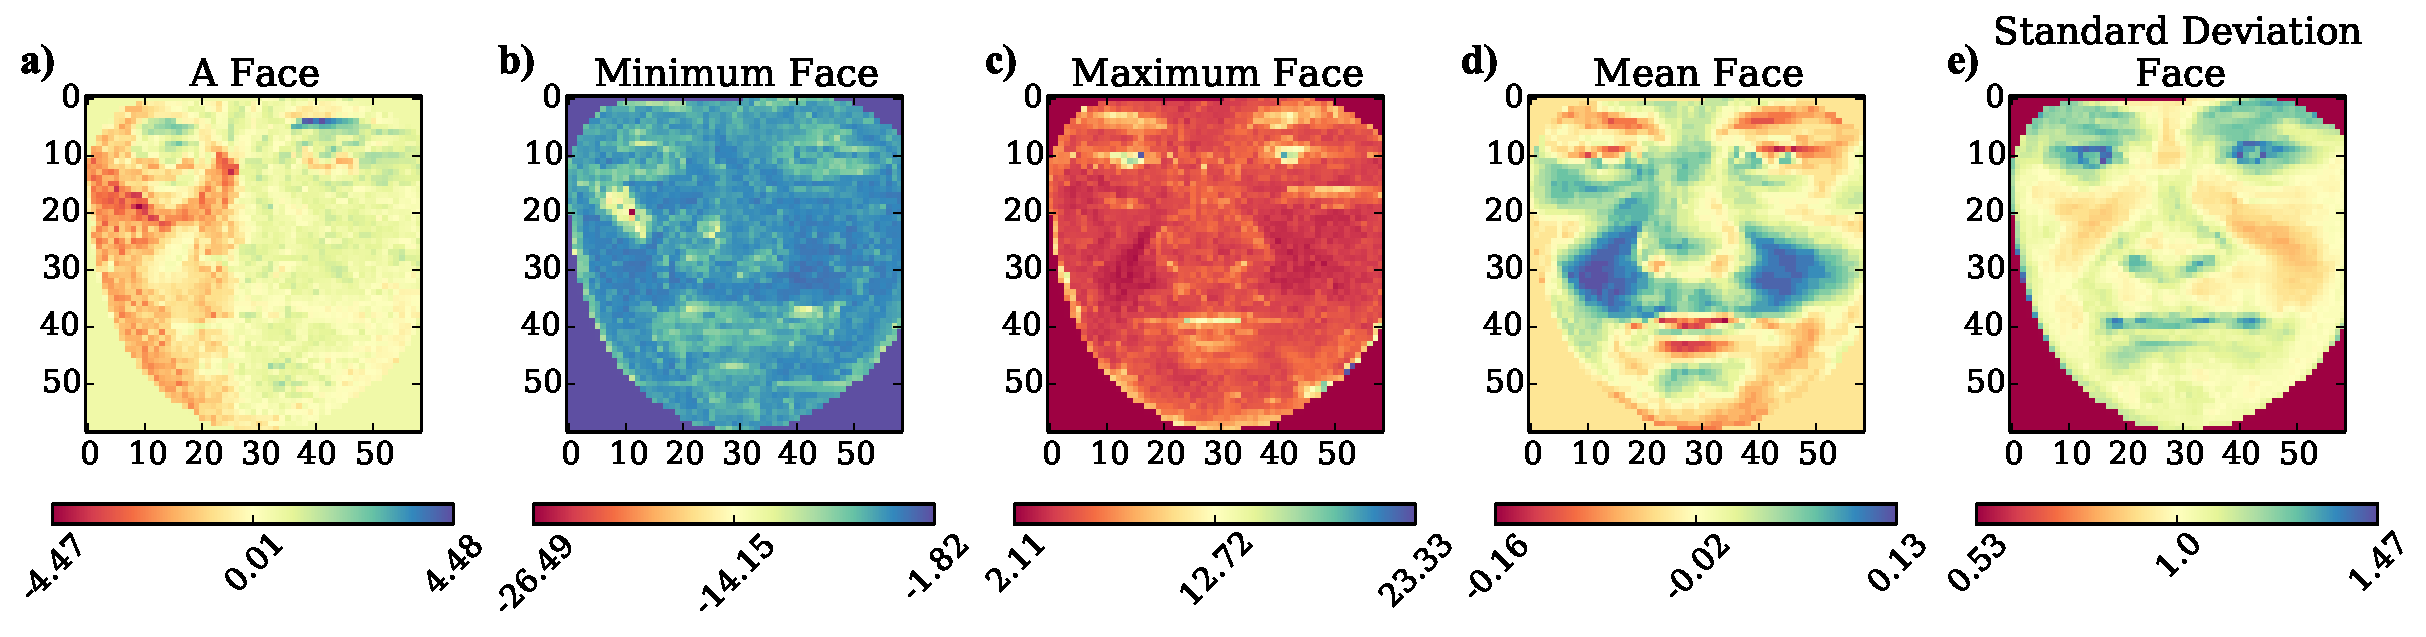
\includegraphics[width =\hsize]{figures/faces_per_subject_contrast_face.pdf}
      \caption{The DISFA dataset with {\bf per subject mean face normalisation and then contrast normalisation} applied.
      Plots {\bf a)}, {\bf b)}, {\bf c)}, {\bf d)} and {\bf e)}
      correspond to a sample face, the minimum, the maximum,
      the mean and the standard deviation values of each pixel across
      the whole dataset. The images were downscaled by a factor of 0.8 before being processed.}
      \label{fig:faces_per_subject_contrast_face} \end{figure}

    %
    %
    %
    %
    %
    \subsection{Masking} \label{sec:mask}
      From figure \ref{fig:faces_none} it is evident some pixels have a maximum and minimum value
      of zero and no deviation. This means there is no information in these areas and hence
      the classifier algorithm would ideally not even know about them. If the network was a set of fully connected layers
      these pixels could just be removed from the system, however convolutional layers require
      rectangular inputs and so a solution is to apply a mask at the level of the cost function.

      As this applies only to the autoencoder who has a cost function (equation \ref{eq:autoencoder_cost}):
      \begin{equation}
          J(\tilde{\mathbf{x}},\tilde{\mathbf{y}})
          = \frac{1}{N}\left |\mathbf{y}(\tilde{\mathbf{x}})-\tilde{\mathbf{x}}\right | ^2
      \end{equation}
      Instead becomes:
      \begin{equation}
          J(\tilde{\mathbf{x}},\tilde{\mathbf{y}})
          = \frac{1}{N}\left |\mathbf{y}(\tilde{\mathbf{x}}) \odot \mathbf{M}-\tilde{\mathbf{x}}\right | ^2
      \end{equation}

      Where M is a two dimensional matrix with elements unity where the dataset is non-zero
      and zero when the dataset is zero for that pixel. Here $\odot$ denotes an element-wise
      product between two matrices.
